\section{Dynamics (formally)}
\subsection{}

\begin{frame}
\frametitleTC{System -- recap and systematisation}
\framesubtitleTC{A mathematical representation (model) of something that evolves}
\myPause
 \begin{columns}
  \column[T]{0.45\textwidth}
   \begin{itemize}[<+-| alert@+>]
   \item[] Simple representation
   \item[] \vspace{2mm}\begin{center}
            \usetikzlibrary{matrix}
\usetikzlibrary{arrows}
\usetikzlibrary{calc}

\tikzstyle{block} = [draw,rectangle,thick,minimum height=3em,minimum width=4em]
\tikzstyle{sum} = [draw,circle,inner sep=0mm,minimum size=2mm]
\tikzstyle{connector} = [->,thick]

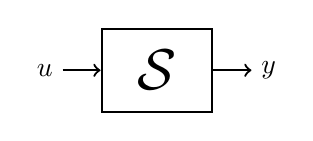
\begin{tikzpicture}[scale=1.00]

\node [left] at (00.00,00.00) (in_u) {$u$};
\node [block] at (01.20,00.00) (S) {{\huge$\mathcal{S}$}};
\draw [connector] (in_u.east) -- (S.west);
\node [right] at (02.40,00.00) (out_y) {$y$};
\draw [connector] (S.east) -- (out_y.west);
\end{tikzpicture}


           \end{center}
           \begin{itemize}[<+-| alert@+>]
           \item[] $u$ -- input(s)
           \item[] $y$ -- output(s)
           \end{itemize}
   \end{itemize}
  \column[T]{0.55\textwidth}
   \begin{itemize}[<+-| alert@+>]
   \item[] Model ingredients
           \begin{itemize}[<+-| alert@+>]
           \item what the system evolves upon:
                 \begin{itemize}[<+-| alert@+>]
                 \item the \TC{continuous time} $t$;
                 \item an integer index $k$ counting some events,
                       frequently called\\the \TC{discrete time}.
                 \end{itemize}
           \item the \TC{evolution law}:
                 \begin{itemize}[<+-| alert@+>]
                 \item $u[t_0,t]\;\rightarrow\;y[t_0,t]$;
                 \item $u[k_0,k]\;\rightarrow\;y[k_0,k]$.
                 \end{itemize}
           \end{itemize}
   \end{itemize}
 \end{columns} \myPause
 \vfill
 \begin{center}
  \vfill \textbf{Is anything missing? \myPause Sometimes, yes.}
 \end{center}
\end{frame}

\begin{frame}
\frametitleTC{\underline{Dynamic} system -- recap and systematisation}
\framesubtitleTC{The most general definition}
\myPause
\begin{center}
 {\Large
 If the knowledge of $u[t_0,t]$ --- or $u[k_0,k]$ \\ \myPause
 allows to determine $y[t_0,t]$ --- or $y[k_0,k]$ \\ \myPause
 the system is said to be \TC{non dynamic},\\ \myPause
 \vspace{1.5mm}\TC{dynamic} otherwise. \myPause
 }
\end{center}
\end{frame}

\begin{frame}
\frametitleTC{Dynamic system -- recap and systematisation}
\framesubtitleTC{Input, output, and \emph{state}}
\myPause
\begin{itemize}[<+-| alert@+>]
\item Non dynamic system:\\
      $y[t_0,t]$ or $y[k_0,k]$ depends only on $u[t_0,t]$ or $u[k_0,k]$.
\item Dynamic system:\\
      $y[t_0,t]$ or $y[k_0,k]$ depends on $u[t_0,t]$ or $u[k_0,k]$,\\
      and on the initial values $x[t_0]$ or $x[k_0]$ of some quantities.
\item These are called the \TC{state variables}, and form the \TC{state (vector)}.
\item The number of state variables is called the \TC{order} of the system.
\end{itemize}
\end{frame}

\begin{frame}
\frametitleTC{Dynamic system -- recap and systematisation}
\framesubtitleTC{How can we express this in mathematical terms?}
\myPause
In several ways. We see the only two relevant for us.\myPause
\begin{itemize}[<+-| alert@+>]
\item Continuous-Time (CT) system:\\
      \begin{displaymath}
       \left\{
        \begin{array}{rl}
         \frac{dx(t)}{dt} &= f \big( x(t),u(t),t  \big) \\
         y(t)             &= g \big( x(t),u(t),t  \big)
        \end{array}
       \right.
      \end{displaymath}
\item Discrete-Time (DT) system:\\
      \begin{displaymath}
       \left\{
        \begin{array}{rl}
         x(k) &= f \big( x(k-1),u(k-1),k  \big) \\
         y(k) &= g \big( x(k),u(k),k  \big)
        \end{array}
       \right.
      \end{displaymath}

\end{itemize}
\end{frame}

\begin{frame}
\frametitleTC{Dynamic system -- recap and systematisation}
\framesubtitleTC{Some more definitions (for both the CT and the DT case)}
\myPause
\begin{itemize}[<+-| alert@+>]
\item \TC{Linear (L)} system:\\
      $f(\cdot,\cdot,\cdot)$ and $g(\cdot,\cdot,\cdot)$ linear in $x$ and $u$.
\item \TC{Time-Invariant (TI)} system:\\
      $f(\cdot,\cdot,\cdot)$ and $g(\cdot,\cdot,\cdot)$ not depending on $t$ or $k$.
\item \TC{Proper} (sometimes, \emph{strictly} proper) system:\\
      $g(\cdot,\cdot,\cdot)$ not depending on $x$,\\
      i.e., the input acts on the output only through the state.
\item \TC{SISO} (Single-Input, Single-Output) system:\\
      $u$ and $y$ -- not necessarily $x$ -- scalars.
\end{itemize}
\end{frame}

\begin{frame}
\frametitleTC{Motion}
\framesubtitleTC{General definition}
\myPause
\centerline{Note: from now on we mostly speak DT, for CT just replace $k$ with $t$.} \myPause
\vspace{3mm}\begin{itemize}[<+-| alert@+>]
\item Initial state + input at a certain start time $\Rightarrow$ motion, i.e.,
      \begin{displaymath}
       \left.
        \begin{array}{l}
         x(k_0) \\ u(k),\,k \geq k_0
        \end{array}
       \right\}
       \quad \Rightarrow \quad
        x(k),y(k),\,k \geq k_0.
      \end{displaymath}
\item We call $x(k)$ and $y(k)$, respectively,
      \begin{itemize}[<+-| alert@+>]
      \item the \TC{state motion}
      \item and the \TC{output motion}
      \end{itemize}
\item [] produced by the initial state $x(k_0)$ and the input $u(k)$, starting\\
      at time $k_0$.
\end{itemize}
\end{frame}

\begin{frame}
\frametitleTC{Motion}
\framesubtitleTC{for the Time-Invariant (TI) case, to which we restrict the scope from now on}
\myPause
\begin{itemize}[<+-| alert@+>]
\item Initial state + input $\Rightarrow$ motion independently of the start time, i.e.,
      \begin{displaymath}
       \left.
        \begin{array}{l}
         x(0) \\ u(k),\,k \geq 0
        \end{array}
       \right\}
       \quad \Rightarrow \quad
        x(k),y(k),\,k \geq 0.
      \end{displaymath}
\item Alternatively, we can say that with TI systems one can set the origin\\
      of the time axis wherever one wants (for convenience, at zero).
\end{itemize}
\end{frame}

\begin{frame}
\frametitleTC{Equilibrium}
\framesubtitleTC{Definition (in the TI case)}
\myPause
\begin{center}
 {\Large
 If there exist some state vectors $\overline{x}$\\ \myPause
 such that $x(0)=\overline{x}$ and $u(k)=\overline{u}$, $k \geq 0$,\\ \myPause
 produce the constant state motion $x(k)=\overline{x}$, $k \geq 0$,\\ \myPause
 then those vectors are called \TC{equilibrium states},\\ \myPause
 or \TC{equilibria} for short,\\ \myPause
 \vspace{1.5mm}corresponding to the constant input $\overline{u}$.
 }
\end{center}
\end{frame}


\begin{frame}
\frametitleTC{Equilibrium}
\framesubtitleTC{Finding equilibrium states and outputs}
\myPause
\begin{itemize}[<+-| alert@+>]
\item A state vector $\overline{x}$ is an equilibrium for a given $\overline{u}$ if the consequent motion is
      $x(k)=x(k-1)=\overline{x}$ $\forall k$.
\item Thus to find equilibria one solves
      \begin{displaymath}
       \overline{x} = f(\overline{x},\overline{u}).
      \end{displaymath}
\item If some equilibrium state exists, and $g(\overline{x},\overline{u})$ does not lose significance,\\
      the result is the corresponding \TC{equilibrium output} $\overline{y}$.
\end{itemize}
\end{frame}

\begin{frame}
\frametitleTC{Stability}
\framesubtitleTC{Preliminaries}
\myPause
\begin{itemize}[<+-| alert@+>]
\item The existence of an equilibrium implies NOTHING on what happens if the system does not start exactly
      at the equilibrium.
\item Discussing this is a matter of \TC{stability}.
\item One can talk about stability of equilibria, motions, and sometimes systems.
\item We define stability for an equilibrium, do not talk about motions,\\
      and move to systems later on.
\end{itemize}
\end{frame}

\begin{frame}
\frametitleTC{Stability}
\framesubtitleTC{Stable equilibrium}
\myPause
\begin{itemize}[<+-| alert@+>]
\item Let $\overline{x}$ be an equilibrium for the constant input $\overline{u}$.
\item Denote by $x_{\Delta}(k)$ the \TC{perturbed motion} produced by
      \begin{itemize}[<+-| alert@+>]
      \item the input $\overline{u}$,
      \item and the \TC{perturbed initial state} $x(0)=\overline{x}+\Delta\overline{x}$.
      \end{itemize}
\item Not that in general, $x_{\Delta}(k)$ will not be constant.
\item Denote by $||x||$ the norm (think here of the Euclidean norm)\\
      of vector $x$.
\end{itemize}
\end{frame}


\begin{frame}
\frametitleTC{Stability}
\framesubtitleTC{Stable equilibrium}
\myPause
\begin{itemize}[<+-| alert@+>]
\item An equilibrium $\overline{x}$ corresponding to the constant input $\overline{u}$ is said to be \TC{stable} if
      \begin{displaymath}
       \forall \varepsilon>0 \;
       \exists \delta_{\varepsilon}>0 \; : \;
       ||\Delta\overline{x}||<\delta_{\varepsilon}
       \Rightarrow ||x_{\Delta}(k)-\overline{x}||<\varepsilon \; \forall k \geq 0.
      \end{displaymath}
\item Interpretation: stable equilibrium means that
      \begin{itemize}[<+-| alert@+>]
      \item no matter how close one wants the \TC{entire} perturbed motion to remain to the equilibrium,
      \item a maximum distance of the initial state from the equilibrium can be\\
            found, that fulfils the desire.
      \end{itemize}
      \item Graphically,
            \begin{center}
             \includegraphics[width=0.60\columnwidth]{./Unit-02/img/StableEq-general.pdf}
            \end{center}
\item If the above does not hold true, the equilibrium is \TC{unstable}.
\end{itemize}
\end{frame}

\begin{frame}
\frametitleTC{Stability}
\framesubtitleTC{Asymptotically stable equilibrium}
\myPause
\begin{itemize}[<+-| alert@+>]
\item An equilibrium $\overline{x}$ corresponding to $\overline{u}$ is said to be \TC{asymptotically stable} if
      \begin{itemize}[<+-| alert@+>]
      \item it is stable,
      \item and \underline{in addition}
            \begin{displaymath}
             \lim_{k\rightarrow\infty} ||x_{\Delta}(k)-\overline{x}||=0.
            \end{displaymath}
      \end{itemize}
      \item Graphically,
            \begin{center}
             \includegraphics[width=0.60\columnwidth]{./Unit-02/img/AsympStableEq-general.pdf}
            \end{center}
\item Clearly asymptotic stability implies stability, but not \emph{vice versa}.
\end{itemize}
\end{frame}

